\section{Software Architecture}
\subsection{What? How?}
\begin{figure}[h]
    \centering
    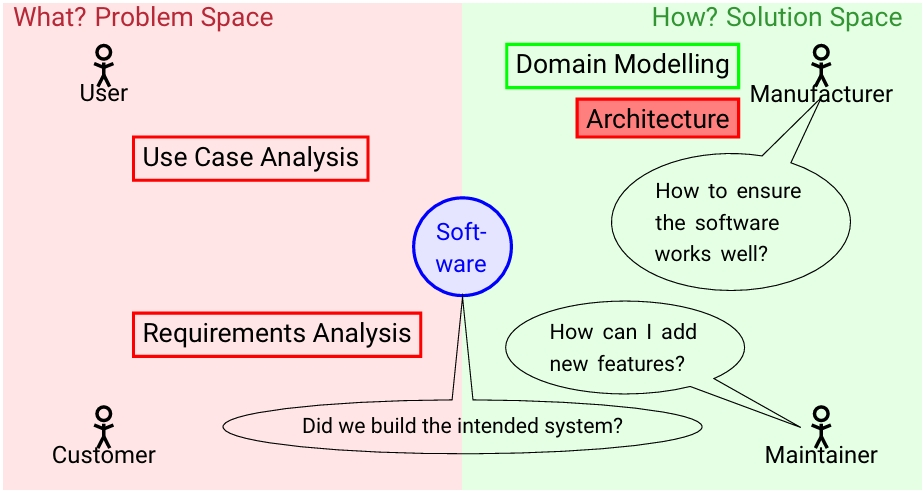
\includegraphics[width=1\textwidth]{Images/Architecture.jpeg}
\end{figure}

\subsubsection*{A Product of its Time}
\begin{defBox}
    Software architecture is a fast evolving area in software engineering
\end{defBox}
Architectures \red{favoured in the past} are \red{now discouraged}\\
\& Architecture \red{discouraged in the past} are \red{now preferred}\\
Changes in the last 10 to 15 years that influenced architecture:
\begin{itemize}
    \item Rise of 
    \begin{itemize}
        \item \red{open interfaces} to easily swap components such as databases
        \item mature \red{open source} tools resulting in significant cost reduction enables, for instance, architectures with large number of databases
    \end{itemize}
    \item \red{Container} technology (lightweight virtualisation)
    \begin{itemize}
        \item containers can be easily added or removed as needed
        \item made architectures like microservices feasible (scalability, elasticity)
    \end{itemize}
\end{itemize}
\begin{infoBox}[title=Veränderungen in den letzten 10-15 Jahren]
    \begin{enumerate}
        \item \fatsf{Offene Schnittstellen (\enquote{Open Interfaces})}
        \begin{itemize}
            \item Es sind Technologien entstanden, die es erleichtern, Komponenten wie Datenbanken auszutauschen, ohne das gesamte System ändern zu müssen.
            \item Dies fördert Modularität, Flexibilität und Anpassungsfähigkeit, da man Technologien schnell wechseln oder anpassen kann.
        \end{itemize}
        \item \fatsf{Ausgereiften Open-Source-Tools}
        \begin{itemize}
            \item Open-Source-Software hat sich stark verbessert und wird heute in Unternehmen breit eingesetzt.
            \item Sie senkt Kosten erheblich und ermöglicht komplexere Architekturen, z.B. solche, die viele separate Datenbanken verwenden.
        \end{itemize}
        \item \fatsf{Container-Technologie (leichtgewichtige Virtualisierung)}
        \begin{itemize}
            \item Container sind eine Technologie, die es ermöglicht, Softwareumgebungen unabhängig zu verpacken. Sie sind leichtgewichtig und benötigen weniger Ressourcen als klassische Virtualisierung (z.B. VMs)
            \item Container können einfach hinzugefügt oder entfernt werden, was System flexibler und effizienter macht
            \item \fatsf{Ergebnis:} Architekturen wie Microservices wurden durch Container erst richtig praktikabel. Diese zeichnen sich durch:
            \begin{itemize}
                \item \fatsf{Skalierbarkeit:} Systeme können nach Bedarf wachsen.
                \item \fatsf{Elastizität:} Ressourcen können flexibel zugeteilt oder freigegeben werden.
            \end{itemize}
        \end{itemize}
    \end{enumerate}
\end{infoBox}
\begin{infoBox}
    Diese Entwicklungen haben Architekturen wie Microservices, Cloud-native Architekturen und andere moderne Ansätze erst ermöglicht. Sie bieten Unternehmer die Möglichkeit, ihre Systeme effizienter, flexibler und kostengünstiger zu gestalten.
\end{infoBox}

\subsubsection*{Dimensions}
\begin{defBox}[title=Software architecture encompasses ...]
    \begin{itemize}
        \item architecture characteristics
        \item architectural style (software system structure)
        \item decisions concerning architecture
        \item design principles
    \end{itemize}
\end{defBox}
\subsubsection*{architecture characteristics}
\begin{center}
    \begin{tabular}{lll}
        \toprule
        Operational & Structural & Cross-Cuting \\
        \midrule
        Availability & Extensibility & Accessibility \\
        Scalability & Maintainability & Privacy \\
        Performance & Leveragibility & Security \\
        ... & Localization & ... \\
        & Configuration & \\
         & ... & \\
        \bottomrule
    \end{tabular}
\end{center}
\begin{infoBox}
    Die Begriffe, die hier aufgelistet sind, beschreiben \fatsf{Qualitätsattribute} einer Softwarearchitektur, die in verschiedene Kategorien unterteilt werden können: \fatsf{Operational, Structural} und \fatsf{Cross-Cutting}. Diese Kategorien helfen, die Anforderungen an ein Softwaresystem besser zu organisieren und zu verstehen.
\end{infoBox}
\begin{infoBox}
    \begin{enumerate}
        \item \fatsf{Operational (Betriebsaspekte)}\\
        Diese Attribute betreffen das Verhalten des Systems während des Betriebs. Sie sind für die Nutzererfahrung und die Systemnutzung entscheidend.
        \begin{itemize}
            \item \fatsf{Availability (Verfügbarkeit):} Wie oft und wie lange steht das System für die Nutzung bereit?
            \item \fatsf{Scalability (Skalierbarkeit):} Wie gut kann das System wachsen, um mit einer steigenden Last umzugehen?
            \item \fatsf{Performance (Leistung):} Wie schnell und effizient führt das System seine Aufgaben aus?
        \end{itemize}
        \item \fatsf{Structural (Strukturelle Aspekte)}\\
        Diese Attribute betreffen die Struktur der Software und wie leicht sie sich an neue Anforderungen anpassen lässt.
        \begin{itemize}
            \item \fatsf{Extensibility (Erweiterbarkeit):} Wie leicht können neue Funktionen hinzugefügt werden?
            \item \fatsf{Maintainability (Wartbarkeit):} Wie einfach ist es, das System zu reparieren, zu verbessern oder zu aktualisieren?
            \item \fatsf{Leveragibility (Wiederverwendbarkeit):} Wie gut können Teile der Architektur in anderen Projekten wiederverwendet werden?
            \item \fatsf{Localization (Lokalisierung):} Unterstützung von Sprache, Währung und kulturellen Präferenzen in verschiedenen Regionen
            \item \fatsf{Configuration (Konfiguration):} Anpassung des Systems durch Benutzer oder Administratoren, ohne des Code zu ändern
        \end{itemize}
        \item \fatsf{Cross-Cutting (Querschnittsaspekte)}\\
        Diese Attribute haben Auswirkungen auf viele Teile des Systems und müssen daher global betrachtet werden.
        \begin{itemize}
            \item \fatsf{Accessibility (Zugänglichkeit):} Wie leicht können Nutzer, einschließlich Menschen mit Behinderungen, auf das System zugreifen?
            \item \fatsf{Privacy (Datenschutz):} Wie schützt das System sensible Informationen der Nutzer?
            \item \fatsf{Security (Sicherheit):} Wie gut schützt das System vor Angriffen und unbefügtem Zugriff?
        \end{itemize}
    \end{enumerate}
\end{infoBox}
\subsubsection*{architectural style (software system structure)}
\begin{figure}[h]
    \centering
    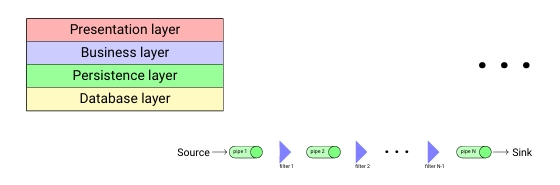
\includegraphics[width=1\textwidth]{Images/architectural style.jpeg}
\end{figure}
\subsubsection*{decisions concerning architecture}
\begin{itemize}
    \item \red{What} \blue{kind} of web framework shall be used?
    \item \red{What} are each layer's responsibilities?
    \item \red{Which} layers can communicate with each other?
    \item \red{What} exchange data formats must be used?
\end{itemize}
\subsubsection*{design principles}
\begin{itemize}
    \item NoSQL databases are the preferred storage option
    \item Immutable data structures are preferred
    \item Use asynchronous messaging between services when possible 
    \item Avoid usage of caching in clients
\end{itemize}
\subsection{Architecture and Design}
\subsubsection*{Demarcation line}
\begin{defBox}[title=Architects are responsible for ...]
    \begin{itemize}
        \item extracting the architecture characteristics from the requirement analysis
        \item choosing a set of styles for the software system
        \item creating the component structure (concise \& coherent parts of a system, above class level)
    \end{itemize}
\end{defBox}
\begin{figure}[h]
    \centering
    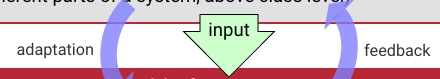
\includegraphics[width=0.5\textwidth]{Images/Demarcation line.jpeg}
\end{figure}
\begin{defBox}[title=Development team is responsible for ...]
    \begin{itemize}
        \item designing the class structure for each component (clss diagrams) (class structure must allow to meet the architecture characteristics)
        \item designing the user interface
        \item writing and testing the source code
    \end{itemize}
\end{defBox}
\begin{defBox}
    Modern architecture is \red{iterative} and incorporates feedback. Supporting \red{software evolution}.
\end{defBox}
\subsection{Architecture Characteristics}
\begin{defBox}[title=Architecture Characteristics]
    An \red{architecture characteristic} meets the following criteria:
    \begin{itemize}
        \item Specifies a \red{non-domain design consideration:} specifies operational and design criteria concerining \red{how to} implement a given requirement
        \item Influences a \red{structural design aspect}: requires the introduction of specific architectural elements (modules, components, ...), not merely \red{best practices} in design/coding
        \item Critical/important that application \red{performs as intended}: meets functional and non-functional requirements
    \end{itemize}
\end{defBox}
Whether a specific characteristic meets the above defined criteria may devend on the context of the software system
\begin{infoBox}
    \begin{enumerate}
        \item \fatsf{Definition eines Architedturmerkmals}\\
        Ein Architekturmerkmal erfüllt die folgenden Kriterien:
        \begin{enumerate}
            \item \fatsf{Es spezifiziert eine nicht-domänenspezifische Disignüberlegung:}
            \begin{itemize}
                \item \fatsf{Was bedeutet das?}
                \begin{itemize}
                    \item Das Merkmal konzentriert sich nicht auf die Geschäftslogik (z.B. das Buchen eines Termins), sondern auf \fatsf{wie} ein bestimmtes Verhalten oder eine Eigenschaft technisch umgesetzt wird.
                    \item Beispiel: Verfügbarkeit, Sicherheit oder Skalierbarkeit sind keine Domänenanforderungen, sondern technische Überlegungen.
                \end{itemize}
            \end{itemize}
            \item \fatsf{Es beeinflusst die strukturelle Gestaltung:}
            \begin{itemize}
                \item \fatsf{Was bedeutet das?}
                \begin{itemize}
                    \item Um das Merkmal zu erfüllen, müssen bestimmte \fatsf{architektonische Elemente} eingeführt werden, wie Module, Komponenten oder Services.
                    \item Es geht nicht nur um die Anwendung von Best Practices, sondern um Entscheidungen, die die gesamte Architektur beeinflussen.
                    \item Beispiel: Für Skalierbarkeit könnte man Microsevices einführen oder Lastenausgleichsmechanismen.
                \end{itemize}
            \end{itemize}
            \item \fatsf{Es ist kritisch/wichtig für die Funktionalität:}
            \begin{itemize}
                \item \fatsf{Was bedeutet das?}
                \begin{itemize}
                    \item Das System muss bestimmte funktionale und nicht-funktionale Anforderungen erfüllen. Ein Architekturmerkmal unterstützt die Umsetzung dieser Anforderungen.
                    \item Beispiel: Ein E-Commerce-System muss \fatsf{hohe Verfügbarkeit} sicherstellen, damit Nutzer jederzeit einkaufen können.
                \end{itemize}
            \end{itemize}
        \end{enumerate}
        \item \fatsf{Kontextabhängigkeit}
        ob ein bestimmtes Merkmal tatsätchlich als Architekturmerkmal gilt, hängt vom \fatsf{Kontext des Softwaresystem} ab:
        \begin{itemize}
            \item \fatsf{Beispiel:}
            \begin{itemize}
                \item Für ein Buchungssystem in einer Arztpraxis könnte \fatsf{Sicherheit} ein zentrales Architekturmerkmal sein.
                \item In einem internen Prototypensystem könnte Sicherheit weniger wichtig sein.
            \end{itemize}
        \end{itemize}
    \end{enumerate}
\end{infoBox}
\subsection{Architectureal Styles}
\subsubsection*{General}
\begin{defBox}[title=Architectural styles ...]
    \begin{itemize}
        \item help to specify the \red{fundamental structure} of a software system
        \item have impact on the appearance of \red{concrete software architectures}
        \item define a system's \red{global properties} such as:
        \begin{itemize}
            \item how distributed components cooperate and exchange data
            \item boundaries of subsystems
        \end{itemize}
    \end{itemize}
\end{defBox}
\begin{defBox}
    Software System are often composed of different architecture styles
\end{defBox}
\subsubsection{Examples}
\begin{defBox}[title=Examples of architectural styles]
    \blue{monolithic}
    \begin{itemize}
        \item \red{Layers}
        \item \red{Pipes and Filters}
        \item \red{Model-View-Controller}
    \end{itemize}
    \blue{distributed}
    \begin{itemize}
        \item \red{Service-Based}
        \item Broker
        \item Microservices
    \end{itemize}
\end{defBox}
\begin{defBox}[title=Choosing an architectural style]
    Choice of architectural style (almost) \red{always} comes with trade-offs.\\
    it is necessity to be aware of these, because additional measures might have to be taken to ensure that all architectuure characteristics are met.
\end{defBox}
\section{Monolithic Architectural Styles}
\begin{figure}[h]
    \centering
    \includegraphics[width=0.5\textwidth]{Images/Architectural Style: Layered.jpeg}
\end{figure}
\begin{infoBox}[title=Topologie und Schichten]
    Die Schichtenarchitektur organisiert Software in aufeinanderfolgende Ebenen (Layers), wobei jede Schicht spezifische Aufgaben übernimmt. Typische Schichten sind:
    \begin{itemize}
        \item \fatsf{Presentation Layer (Präsentationsschicht):} Interagiert mit Benutzern (z.B. UI oder API)
        \item \fatsf{Business Layer (Geschäftslogik):} Beinhaltet die Kernlogik des Systems und verarbeitet Daten gemäß den Anforderungen
        \item \fatsf{Persistence Layer (Datenpersistenz):} Verantwortlich für die Kommunikation mit der Datenbank
        \item \fatsf{Database Layer (Datenbankschicht):} Speicherort für die tatsächlichen Daten
    \end{itemize}
\end{infoBox}
\begin{defBox}[title=Topology]
    Number (and names) of layers not fixed. Some architectures ...
    \begin{itemize}
        \item unify business and persistence layer (business objects create SQL statements themselves)
        \item use additional layers (e.g., service) to enable reuse or restrict access
    \end{itemize}
\end{defBox}
\begin{infoBox}[title=Topologie: Anpassbarkeit der Schichten]
    \begin{itemize}
        \item \fatsf{Anzahl und Namen der Schichten:} Sind nicht fixiert, können je nach Anforderungen angepasst werden.
        \item \fatsf{Verschmelzung von Schichten:} Manche Architekturen kombinieren z.B. die \fatsf{Business}- und \fatsf{Persistence Layer}, indem Geschäftsobjekte direkt SQL-Statements erstellen.
        \item \fatsf{Zusätzliche Schichte:} Einige Architekturen fügen Schichten wie eine \fatsf{Service Layer} hinzu, um Wiederverwendung zu ermöglichen oder den Zugriff einzuschränken.
    \end{itemize}
\end{infoBox}
\begin{defBox}[title=Decisions concerning architecture]
    \begin{itemize}
        \item Definition of responsibilities for each layer
        \item Layer type (open or closed)
        \begin{itemize}
            \item Top-Down request must pass through closed layers, can skip open layers
            \item Open layers improve performance (less call chining), but reduce isolation
        \end{itemize}
    \end{itemize}
\end{defBox}
\begin{infoBox}[title=Entscheidungen bei der Architektur]
    \begin{itemize}
        \item \fatsf{Verantwortlichkeit jeder Schicht:} Jede Schicht hat klar definierte Aufgaben und sollte keine Verantwortung einer anderen Schicht übernehmen.
        \item \fatsf{Schichtentyp: Open vs. Closed Layers}
        \begin{itemize}
            \item \fatsf{Closed Layers (Geschlossene Schichten):} Alle Anfragen müssen die Schichten der Reihe nach durchlaufen.\\
            Vorteil: Klare Isolation der Verantwortlichkeit.\\
            Nachtiel: Kann die Leistung beeinträchtigen.
            \item \fatsf{Open Layers (Offene Schichten):} Anfragen können Schichten überspringen.\\
            Vorteil: Verbesserte Leistung (weniger Call-Chaining).\\
            Nachteil: Reduzierte Isolation und Wartbarkeit.
        \end{itemize}
    \end{itemize}
\end{infoBox}
\begin{defBox}[title=Trade Offs (selection)]
    + Simplicity and Cost
    + Reliability (medium)
    - Elasticity and scalability 
    - Performance: parallelization not inherently supported by architecture
    - Availability: usually long startup time / long mean time to recovery
\end{defBox}
\begin{infoBox}[title=Architectural Style: Layered (Trade-offs)]
    \begin{itemize}
        \item \fatsf{Vorteile:}
        \begin{itemize}
            \item \fatsf{Simplicity and Cost (Einfachheit und Kosten):} Einfach zu implementieren und günstig.
            \item \fatsf{Reliability (Zuverlässigkeit):} Mittlere Zuverlässigkeit durch klare Trennung der Schichten.
        \end{itemize}
        \item \fatsf{Nachteile:}
        \begin{itemize}
            \item \fatsf{Elasticity and Scalability (Elastizität und Skalierbarkeit):} Nicht optimiert für parallele Verarbeitung.
            \item \fatsf{Performance:} Kann bei vielen Schichten leiden.
            \item \fatsf{Availability (Verfügbarkeit:)} Lange Startzeiten und Ausfallwiederherstellung.
        \end{itemize}
    \end{itemize}
\end{infoBox}
\begin{defBox}[title=Summary]
    \begin{itemize}
        \item Technologically partitioned, \red{not} domain partitioned style
        \item Works well for \red{small} to \red{medium-size} applications
        \item Serves as \red{initial} architecture, can be changed later
        \item \red{Problematic:} Often not conscious decition, but result of Conway's law (Design reflicts organisational structure of the company)
    \end{itemize}
\end{defBox}
\begin{infoBox}[title=Zusammenfassung]
    \begin{itemize}
        \item \fatsf{Technologie Partitionierung:} \\
        Die Architektur ist nach technischen Aspekten (z.B. Datenbank, UI) gegliedert, nicht nach Domänenlogik.
        \item \fatsf{Eignung:}
        \begin{itemize}
            \item Gut geeignet für kleine bis mittelgroße Anwendungen.
            \item Häufig als Ausgangsarchitektur gewählt, später eventuell geändert.
        \end{itemize}
        \item \fatsf{Problem:}\\
        Oft nicht bewusst entschieden, sondern durch \fatsf{Conway's Law} bedingt: \enquote{Das Design eines Systems reflektiert die Organisationsstruktur des Unternehmens.}
    \end{itemize}
\end{infoBox}

\clearpage
\subsubsection*{Pipes and Filters}
\begin{figure}[h]
    \centering
    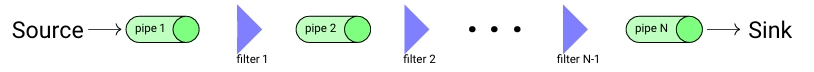
\includegraphics[width=1\textwidth]{Images/Pipes and Filters.jpeg}
\end{figure}
\begin{defBox}[title=Main topology]
    \begin{itemize}
        \item \red{Pipes}
        \begin{itemize}
            \item are \red{unidirectional, point-to-point channels} from a data source to a target
            \item allow any data format (i.e. not restricted by style); formats supporting smaller data chunks are preferred for better performance/throughput
        \end{itemize}
        \item \red{Filters} are
        \begin{itemize}
            \item \red{self-contained} and \red{independent} from other filters
            \item \red{stateless}, intuitively this means its operation does not depend on the past and should realize exactly \red{one} task 
        \end{itemize}
        \item Different kinds of \red{filters}
        \begin{itemize}
            \item \red{Producer:} Source of the data
            \item \red{Transformer:} (i) Receinves data from its input channel(s); (ii) performs operations on the data and (iii) forwards the result via its output channel
            \item \red{Consumer:} Sink of the data where it is output on the display, written to a file or database
        \end{itemize}
    \end{itemize}
\end{defBox}
\begin{infoBox}[title=Hauptkomponenten und ihre Funktionen]
    \begin{enumerate}
        \item \fatsf{Pipes (Kanäle):}
        \begin{itemize}
            \item \fatsf{Eigenschaften:}
            \begin{itemize}
                \item Datenflüsse sind \fatsf{unidirektional} (von einer Quelle zu einem Ziel)
                \item Sie verbinden die Filter miteinander
                \item Unterstützen beliebige Datenformate, bevorzugen jedoch Formate, die in \fatsf{kleinen Datenblöcken} verarbeitet werden können (verbessert die \fatsf{Performance und den Durchsatz})
            \end{itemize}
            \item \fatsf{Zweck:} Dienen als Transportmechanismus, um Daten zwischen den Filtern zu übertragen
        \end{itemize}
        \item \fatsf{Filters (Filter):}
        \begin{itemize}
            \item \fatsf{Eigenschaften:}
            \begin{itemize}
                \item Sind \fatsf{autonom} (arbeiten unabhängig von anderen Filtern)
                \item \fatsf{Zustandslos:} Sie speichern keine Informationen über vorherige Verarbeitungen. Jede Ausführung hängt vur von der aktuellen Eingabe ab
                \item \fatsf{Aufgabenorientiert:} Jeder Filter erfüllt genau \fatsf{eine Aufgabe}
            \end{itemize}
            \item \fatsf{Funktion:} Emjpfangen Daten über Eingabekanäle, verarbeiten sie, und senden die Ergebnisse über Ausgabekanäle weiter
        \end{itemize}
    \end{enumerate}
\end{infoBox}
\begin{infoBox}[title=Arten von Filtern]
    \begin{enumerate}
        \item \fatsf{Producer (Erzeuger):}
        \begin{itemize}
            \item Ursprung der Daten
            \item Beispiel: Ein Sensor, der Messwerte liefert
        \end{itemize}
        \item \fatsf{Transformer (Transformator):}
        \begin{itemize}
            \item \fatsf{Aufgaben:}
            \begin{enumerate}
                \item Daten über einen Eingabekanal empfangen
                \item Verarbeitungen durchführen (z.B. Transformation, Filterung, Berechnungen)
                \item Ergebnisse über den Ausgabekanal weiterleiten
            \end{enumerate}
            \item Beispiel: Ein Bildfilter, der Kontrastanpassungen durchführt.
        \end{itemize}
        \item \fatsf{Consumer (Verbraucher):}
        \begin{itemize}
            \item Endpunkt der Daten
            \item Beispiel: Eine Datenbank, in die Ergebnisse geschrieben werden, oder ein Anzeigesystem, das Ergebnisse darstellt
        \end{itemize}
    \end{enumerate}
\end{infoBox}
\begin{infoBox}[title=Zusammenfassung der Topologie]
    \begin{itemize}
        \item \fatsf{Pipes and Filters} folgt einem \fatsf{linearen oder verzweigten Ablauf:}
        \begin{itemize}
            \item Daten fließen von einem \fatsf{Producer} durch eine Reihe von \fatsf{Transformern} bis zu einem \fatsf{Consumer}
        \end{itemize}
        \item \fatsf{Vorteile:}
        \begin{itemize}
            \item \fatsf{Modularität:} Einfaches Hinzufügen oder Austauschen von Filtern
            \item \fatsf{Wiederverwendbarkeit:} Filter können unabhängig voneinander entwickelt werden
            \item \fatsf{Parallelität:} Datenströme können unabhängig verarbeitet werden, was die Leistung steigert.
        \end{itemize}
        \item \fatsf{Einschränkungen:}
        \begin{itemize}
            \item Kann ineffizient sein, wenn große Datenmengen verarbeitet werden oder Filter komplexe Aufgaben übernehmen
        \end{itemize}
    \end{itemize}
    Dieses Muster eignet sich besonders für Szenarien wie \fatsf{Datenverarbeitung in Echtzeit, Streaming} oder \fatsf{Bild-/Audioverarbeitung}
\end{infoBox}
\begin{figure}[h]
    \centering
    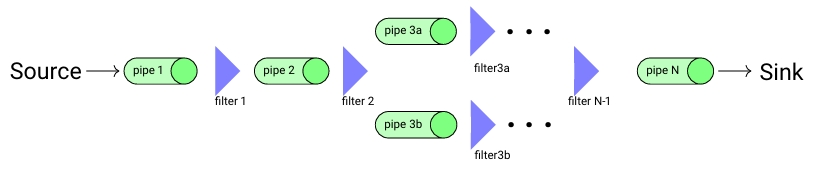
\includegraphics[width=1\textwidth]{Images/Variant topology.jpeg}
\end{figure}
\begin{defBox}[title=Variant topology (branching)]
    Additional kind of filter\\
    \red{Tester:} (i) Receives input; (ii) tests whether data satisfies certain conditions and (iii) redirects data according to outcome o tests to different output channels
\end{defBox}
\begin{infoBox}[title=Topologie]
    Die Topologie von Pipes and Filters sieht so aus:\\
    \fatsf{Quelle $\rightarrow$ Pipe 1 $\rightarrow$ Filter 1 $\rightarrow$ Pipe 2 $\rightarrow$ ... $\rightarrow$ Pipe N $\rightarrow$ Ziel}
    \begin{itemize}
        \item \fatsf{Quelle:} Der Startpunkt der Daten (z.B. eine Datei oder ein Eingabestream).
        \item \fatsf{Ziel:} Der Endpunkt, an dem die verarbeiteten Daten gespeichert, angezeigt oder weitergeleitet werden.
    \end{itemize}
\end{infoBox}
\begin{infoBox}[title=Beispielanwendung]
    \fatsf{Bildverarbeitung}
    \begin{itemize}
        \item \fatsf{Quelle:} Ein hochgeladenes Bild.
        \item \fatsf{Filter 1 (Weißabgleich):} Passt die Farben an.
        \item \fatsf{Filter 2 (Rauschunterdrückung):} Entfernt Bildrauschen.
        \item \fatsf{Filter 3 (JPEG-Kompression:)} Komprimiert das Bild, bevor es gespeichert wird.
        \item \fatsf{Ziel:} Speichert das bearbeitete Bild auf einer Festplatte.
    \end{itemize}
\end{infoBox}
\subsection{Architectural Style: Model-View-Controller (MVC)}
\subsubsection*{Main Topology}
\begin{defBox}
    Fundamental struchtural organization for interactive software systems
\end{defBox}
\begin{figure}[h]
    \centering
    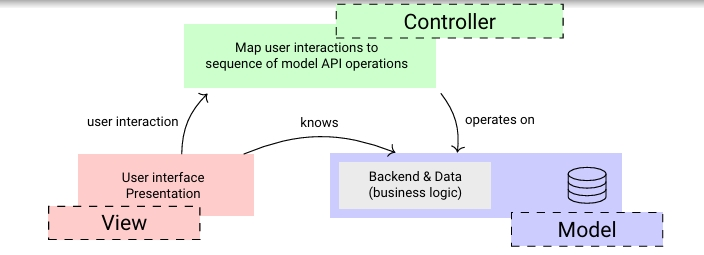
\includegraphics[width=1\textwidth]{Images/Main Topology.jpeg}
\end{figure}
\begin{defBox}[title=Main Topology]
    \begin{itemize}
        \item Separates system in three modules: Model-View-Controller
        \begin{itemize}
            \item \red{Model:} business logic and data storage independent of
            \begin{itemize}
                \item input behavior
                \item output representation
            \end{itemize}
            \item \red{View:} presentation of (parts of) the model data to the user
            \begin{itemize}
                \item data obtained from model
                \item frequently more than one (different kind of) view
            \end{itemize}
            \item \red{Controller:} translates user interactions to operations on the model
            \begin{itemize}
                \item each view is associated to a controller
                \item all interactions via controller
            \end{itemize}
        \end{itemize}
        \item Controller and View are \red{directly coupled with the Model}
        \item Model is \red{not directly coupled with the Controller or the View}
    \end{itemize}
\end{defBox}

\subsubsection*{Change Propagation}
\begin{figure}[h]
    \centering
    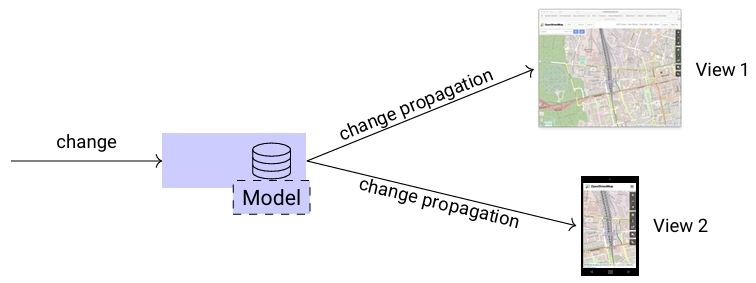
\includegraphics[width=1\textwidth]{Images/Change Propagation.jpeg}
\end{figure}
\begin{defBox}[title=Change Propagation]
    A \red{change propagation mechanism} ensures consistency between the user interface and the model (Often implemented using the Observer/Publisher-Subscriber pattern; see later lacture)
\end{defBox}
\begin{defBox}[title=Basic Idea]
    \begin{itemize}
        \item Views \red{register} themselves at a model (Controllers, whose behavior depends on the model state, register themselves also at the model)
        \item Model \red{notifies} registered view objects upon change
    \end{itemize}
\end{defBox}

\clearpage
\subsubsection*{CaSh-Static structure}
\begin{figure}[h]
    \centering
    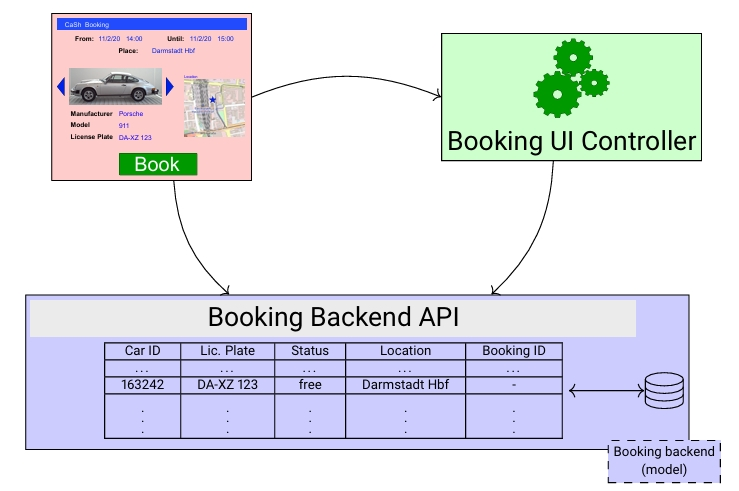
\includegraphics[width=0.65\textwidth]{Images/CaSh-Static structure.jpeg}
\end{figure}

\subsubsection*{CaSh - Dynamic}
\begin{figure}[h]
    \centering
    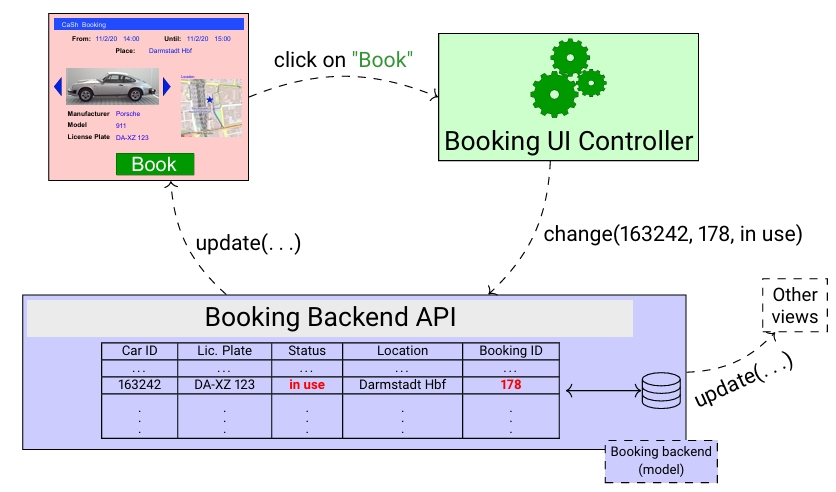
\includegraphics[width=0.75\textwidth]{Images/CaSh-Dynamic.jpeg}
\end{figure}

\subsubsection*{Applicability and Trade-Offs}
\begin{defBox}[title=When to use MVC]
    Applicaton is interactive and:
    \begin{itemize}
        \item the model data should be presented in different ways
        \item number and kind of views are not fixed (and/or unknown)
        \item display and application behavior must reflect data changes immediately
        \item changing and porting the UI should not affect the application's core
    \end{itemize}
\end{defBox}
\begin{defBox}[title=Trade-Offs]
    \begin{enumerate}
        \item Update proliferation, \red{but} not all views are interested in all changes
        \item Increase in complexity ue to separate view and controller components without gaining much flexibility
        \item High dependency (coupling)betwenn view and controller
    \end{enumerate}
\end{defBox}
\begin{infoBox}[title=Wann sollte MVC verwendet werden?]
    \begin{enumerate}
        \item \fatsf{Interaktive Anwendungen:}
        \begin{itemize}
            \item Wenn Benutzereingaben Änderungen an Daten erfordern und diese sofort in der Oberfläche (UI) sichtbar sein müssen
        \end{itemize}
        \item \fatsf{Mehrere Darstellungen:}
        \begin{itemize}
            \item Wenn dieselben Daten (\fatsf{Model}) in \fatsf{verschiedenen Ansichten oder Formaten} dargestellt werden sollen (z.B. als Liste oder Diagramm)
        \end{itemize}
        \item \fatsf{Dynamische Ansichten:}
        \begin{itemize}
            \item Wenn die \fatsf{Anzahl und Art der Ansichten nicht festgelegt} oder im Voraus bekannt sind und sich im Laufe der Zeit ändern können
        \end{itemize}
        \item \fatsf{Trennung von Logik und UI:}
        \begin{itemize}
            \item Wenn das Ändern oder Portieren der \fatsf{Benutzeroberfläche (UI)} unabhängig vom Kern der Anwendung erfolgen soll
        \end{itemize}
    \end{enumerate}
\end{infoBox}
\begin{infoBox}[title=Trade-offs von MVC]
    \begin{enumerate}
        \item \fatsf{Update-Welle:}
        \begin{itemize}
            \item \fatsf{Problem:} Änderungen am Model benachrichtigen \fatsf{alle Views}, selbst wenn nicht alle die Änderung benötigen
            \item \fatsf{Auswirkung:} Dies kann zu unnötigem Aufwand und Leistungseinbußen führen
        \end{itemize}
        \item \fatsf{Erhöhte Komplexität:}
        \begin{itemize}
            \item \fatsf{Problem:} Die strikte Trennung zwichen Model, View und Controller führt zu mehr \fatsf{Komponenten}, was die Entwicklung komplizierter macht
            \item \fatsf{Auswirkung:} Wenn Flexibilität nicht entscheidend ist, kann die zusätzliche Komplexität unnötig sein
        \end{itemize}
        \item \fatsf{Abhängigkeit zwischen View und Controller:}
        \begin{itemize}
            \item \fatsf{Problem:} View und Controller sind oft \fatsf{stark gekoppelt}, was die Wiederverwendbarkeit einschränkt und Abhängigkeiten erhöht
            \item \fatsf{Auswirkung:} Änderungen an einer Komponente können die andere beeinträchtigen, was die Modularität verringert
        \end{itemize}
    \end{enumerate}
\end{infoBox}

\clearpage
\section{Distributed Architectural Styles}
\subsection{Architectural Style: Service-Based}
\subsubsection*{Main Topology}
\begin{figure}[h]
    \centering
    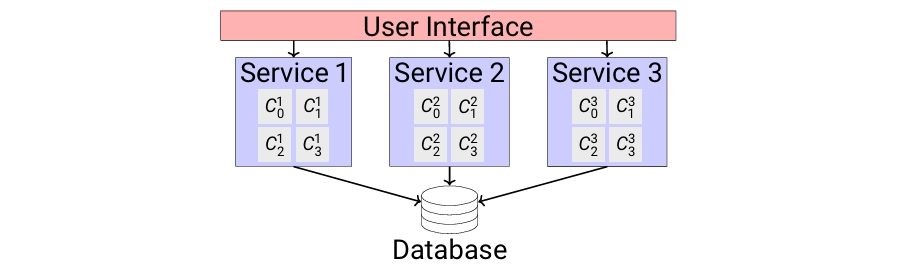
\includegraphics[width=1\textwidth]{Images/Service-Based.jpeg}
\end{figure}
\begin{defBox}[title=Main Topology]
    \begin{itemize}
        \item One monolithic user interface for all services
        \item Each service i is composed of different components $C^{i}_{j}$
        \item Services share a common database
    \end{itemize}
\end{defBox}
\begin{infoBox}[title=Haupttopologie des Service-Based-Stils]
    \begin{enumerate}
        \item \fatsf{Monolithische Benutzeroberfläche (UI):}
        \begin{itemize}
            \item In dieser Architektur gibt es \fatsf{ein zentrales Benutzerinterface}, das alle Dienste bedient. Das bedeutet, dass der Benutzer über eine einzige Oberfläche mit allen Services interagiert
            \item Diese Oberfläche ist dafür verantwortlich, Anfragen an die verschiedenen Services zu stellen und die Ergebnisse entsprechend anzuzeigen
        \end{itemize}
        \item \fatsf{Services und ihre Komponenten:}
        \begin{itemize}
            \item Jeder \fatsf{Service} (z.B. für eine bestimmte Funktion wie Benutzerverwaltung oder Zahlungsabwicklung) besteht aus mehreren \fatsf{Komponenten}
            \item Jede Komponente innerhalb eines Services ist für eine bestimmte Aufgabe zuständig, aber alle zusammen ermöglichen sie die vollständige Funktionalität des Services
            \item Die Komponenten innerhalb eines Services arbeiten eng zusammen, um eine konsistente Dienstleistung bereitzustellen
        \end{itemize}
        \item \fatsf{Gemeinsame Datenbank:}
        \begin{itemize}
            \item Alle \fatsf{Services} in diesem Modell teilen sich eine \fatsf{gemeinsame Datenbank}
            \item Das bedeutet, dass alle Services auf dieselben Daten zugreifen und diese verwalten. Es gibt keine separate Datenbank für jeden Service
            \item Diese Struktur kann dazu führen, dass es eine \fatsf{engere Kopplung} zwischen den Services und der Datenbank gibt, was manchmal die Skalierbarkeit und Flexibilität einschränken kann, jedoch einfacher für klienere bis mittlere Systeme ist
        \end{itemize}
    \end{enumerate}
\end{infoBox}

\subsubsection*{Topology Variants}
\begin{defBox}[title=Non-monolithic user interfaces]
    \begin{itemize}
        \item Domain-based user interface
        \item Service-based user interface (one UI per service; not shown)
    \end{itemize}
\end{defBox}
\begin{infoBox}[title=Nicht-monolitische Benutzeroberflächen]
    \begin{enumerate}
        \item \fatsf{Domänenbasierte Benutzeroberfläche:}
        \begin{itemize}
            \item Bei diesem Ansatz wird die Benutzeroberfläche (UI) basierend auf den \fatsf{Domänen} (also den Hauptbereichen der Anwendung, wie z.B. Kundenmanagement, Bestllverwaltung, etc.) strukturiert
            \item Jede Domäne erhält eine eigene Benutzeroberfläche, die spezifische Funktionen und Interaktionen für diese Domäne bereitstellt
            \item Die Vorteile liegen in der besseren \fatsf{Trennung der Anliegen} und einer klareren Struktur der UI, da jede Domäne ihr eigenes UI hat
        \end{itemize}
        \item \fatsf{Service-basierte Benutzeroberfläche:}
        \begin{itemize}
            \item In diesem Fall gibt es für \fatsf{jeden Service} eine separate Benutzeroberfläche. Jeder Service hat sein eigenes I, das auf die Funktionalität dieses Services fokussiert ist
            \item Diese Architektur ermöglicht eine \fatsf{sehr hohe Flexibilität} und Modularität, da jeder Service unabhängig von den anderen seine eigene UI-Logik hat
        \end{itemize}
        \item \fatsf{Vorteil:} Veränderungen oder Erweiterungen eines Services können vorgenommen werden, ohne die UI anderer Services zu beeinträchtigen
        \item \fatsf{Nachteil:} Es kann zu einer erhöhten Komplexität führen, da mehrere UIs verwaltet werden müssen
    \end{enumerate}
\end{infoBox}
\begin{figure}[h]
    \centering
    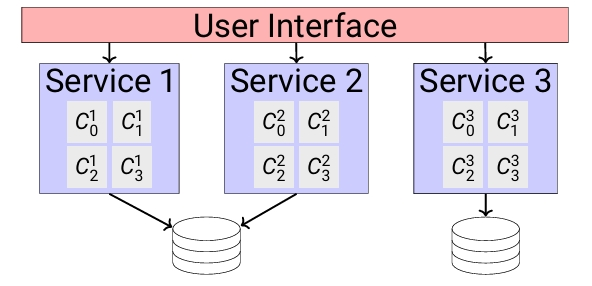
\includegraphics[width=0.9\textwidth]{Images/Database Location.jpeg}
\end{figure}
\begin{defBox}[title=Database Location]
    \begin{itemize}
        \item Service-local databases
        \begin{itemize}
            \item Data owned by one service (opne service type)\\
            all queries and changes must use service API
            \item Structure supports data consistency and easier scalability
        \end{itemize}
        \item Miced configuration of shared and service-local databases (shown)
        \begin{itemize}
            \item Shared databases (esp. shared schemas) require coordination
            \item Data ownership must be clearly defined \\
            Target: One service has write permissions, multiple may read
        \end{itemize}
    \end{itemize}
\end{defBox}
\begin{infoBox}[title=Datenbankkonfigurationen]
    \begin{enumerate}
        \item \fatsf{Service-lokale Datenbanken:}
        \begin{itemize}
            \item In diesem Modell besitzt jeder \fatsf{Service sein eigene Datenbank}. Das bedeutet, dass jeder Service für seine Daten verantwortlich ist und sämtliche \fatsf{Abfragen und Änderungen} nur über die API des jeweiligen Services durchgeführt werden
            \item \fatsf{Vorteil:} Durch die Trennung der Datenbank je Service wird eine klare \fatsf{Datenkonsistenz} gewährleistet. Zudem ist diese Struktur sehr \fatsf{skalierbar,} da Services unabhängig voneinander skaliert werden können, ohne die Datenbank jedes anderen Services zu beeinflussen
            \item \fatsf{Nachteil:} Es könnte eine größere \fatsf{Datenwiederholung} geben, wenn mehrere Services ähnliche Daten benötigen
        \end{itemize}
        \item \fatsf{Gemischte Konfiguration von geteilten und Service-lokalten Datenbanken:}
        \begin{itemize}
            \item In dieser Konfiguration gibt es sowohl \fatsf{geteilte Datenbanken} (die von mehreren Services genutzt werden) als auch \fatsf{lokale Datenbanken} für bestimmte Services
            \item \fatsf{Vorteil:} Diese Struktur bietet eine gewisse \fatsf{Flexibilität}, da mehrere Services auf dieselben Daten zugreifen können. Sie erfordert jedoch eine sorgfältige \fatsf{Koordination} bei der Verwaltung der gemeinsamen Daten.
            \item \fatsf{Herausforderung:} Der \fatsf{Datenbesitz} muss klar definiert werden, um sicherzustellen, dass nur ein Service \fatsf{Schreibrechte} auf die Daten hat, während andere Services nur \fatsf{Lesezugriff} erhalten. Diese klare Definition ist notwendig, um \fatsf{Datenkonsistenz} und Konflikte zu vermeiden
            \item \fatsf{Nachteil:} Besonders bei \fatsf{gemeinsam genutzten Datenbanken (z.B. bei geteilten Schemata)} ist eine strenge \fatsf{Koordination und Synchronisation} erforderlich, um sicherzustellen, dass keine Dateninkonsistenzen oder Konflikte zwischen den Services entstehen
        \end{itemize}
    \end{enumerate}
\end{infoBox}
\subsubsection*{CaSh}
\begin{figure}[h]
    \centering
    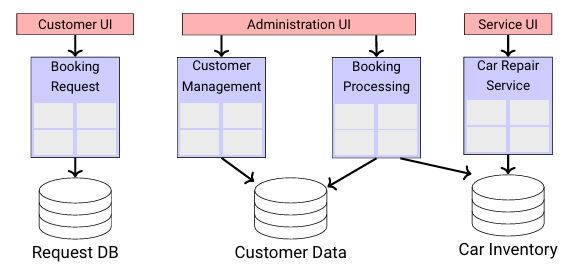
\includegraphics[width=0.9\textwidth]{Images/A service-based architecture for CaSh.jpeg}
\end{figure}
\begin{defBox}[title=A service-based architecture for CaSh]
    \begin{itemize}
        \item Customer UI uses \red{Booking Request} service to generate a booking request
        \item Booking request sent to \red{Booking Processing} service
        \item Service accessible for customer has no direct access to company databases (architecture supports security aspects)
    \end{itemize}
\end{defBox}
\subsubsection*{CaSh - Service Structure}
\begin{figure}[h]
    \centering
    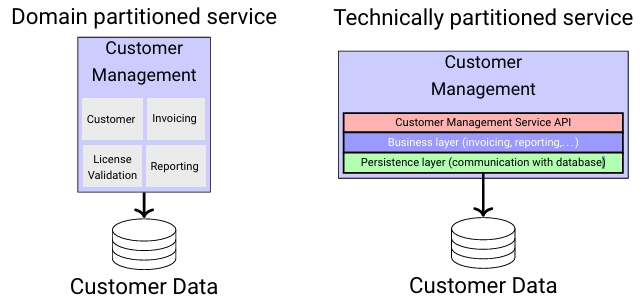
\includegraphics[width=1\textwidth]{Images/CaSh - Service Structure.jpeg}
\end{figure}
\begin{defBox}[title=CaSh: Two alternatice service architectures]
    \begin{itemize}
        \item \red{Domain partitioned} service: components realize domain specific tasks
        \item \red{Technically partitioned} service: components organized as layered structure
    \end{itemize}
\end{defBox}
\begin{infoBox}
    \begin{itemize}
        \item \fatsf{Domain-partitionierte Architektur} ist ideal für Systeme, bei denen die \fatsf{geschäftlichen Domänen} voneinander getrennt sind und klare Verantwortlichkeiten bestehen. Es eignet sich gut für \fatsf{business-orientierte Anwendungen}
        \item \fatsf{Technisch partitionierte Architektur} (Schichtenarchitektur) ist sinnvoll für Anwendungen, bei denen die \fatsf{technischen Aspekte} wie Datenhaltung, Geschäftslogik und Benutzeroberfläche klar voneinander getrennt werden müssen. Es eignet sich gut für \fatsf{technologisch komplexe Systeme}
    \end{itemize}
\end{infoBox}
\clearpage
\section{Wrapping Up}
\subsection{Choosing an Architectural Style}
\subsubsection*{Influences}
\begin{figure}[h]
    \centering
    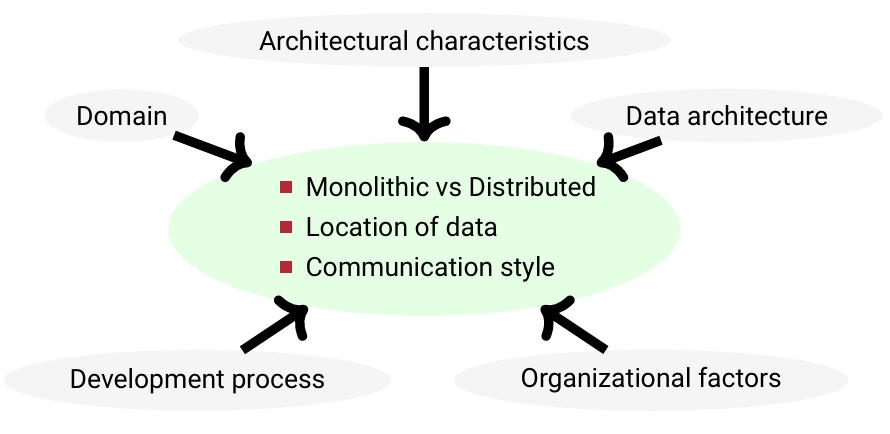
\includegraphics[width=0.9\textwidth]{Images/Choosing an Architectural Style.jpeg}
\end{figure}

\subsection{Decisions Concerning Architecture}
\subsubsection*{Soft Skills}
\begin{defBox}[title=Fear of the wrong decision]
    Decision is avoided/deferred out of fear to make the wrong choice\\
    Possible solution:
    \begin{itemize}
        \item make decistion at \enquote{last \red{responsible} moment}\\
        at a time early enough so that the missing decision does not cause delay to other work
        \item stay clase to development team to be able to react to problems
    \end{itemize}
\end{defBox}
\begin{defBox}[title=Never ending discussions]
    Decision discussed over and over again because reason \red{why} is not known
\end{defBox}
\begin{defBox}[title=Architecture not implemented]
    Architecture not implemented by developers because decisions are not known
\end{defBox}
Both problem are essentially about documentation and communication
\begin{itemize}
    \item Document decisions at a well-known and suitable place
    \begin{itemize}
        \item Formal document
        \item Better: wiki with attached issue tracker used by development team
    \end{itemize}
    \item Choose appropriate media to cummunicate (changes to) decisions
    \item Keep messages concise, refer to wiki/issue tracker/document for details
\end{itemize}
\begin{infoBox}[title=Entscheidungen zur Architektur: Herausforderungen und Lösungen]
    Architekturentscheidungen sind ein zentraler Bestandteil der Softwareentwicklung. Dabei können jedoch typische Herausforderungen auftreten, die durch gezielte Maßnahmen adressiert werden sollten:
    \begin{enumerate}
        \item \fatsf{Angst vor falschen Entscheidungen}
        \begin{itemize}
            \item \fatsf{Problem:} Entscheidungen werden vermieden oder verzögert, aus Angst, eine falsche Wahl zu treffen
            \item \fatsf{Konsequenzen:} Verzögerungen in der Entwicklung, Unsicherheit im Team, mangelnde Fortschritte
            \item \fatsf{Lösungen:}
            \begin{itemize}
                \item \fatsf{Entscheidung zum \enquote{last responsible moment} treffen:}
                \begin{itemize}
                    \item Entscheidungen so spät wie möglich, aber rechtzeitig treffen, damit keine Verzögerungen im Projekt entstehen
                \end{itemize}
                \item \fatsf{Nähe zum Entwicklungsteam:}
                \begin{itemize}
                    \item Enger Kontakt ermöglicht, frühzeitig auf Probleme zu reagieren und fundierte Entscheidungen zu treffen
                \end{itemize}
            \end{itemize}
        \end{itemize}
        \item \fatsf{Endlose Diskussionen}
        \begin{itemize}
            \item \fatsf{Problem:} Entscheidungen werden wiederholt diskutiert, da die Gründe für die Entscheidung nicht klar sind
            \item \fatsf{Konsequenzen:} Zeitverlust, ineffizientes Arbeiten, Verzögerungen bei der Umsetzung
            \item \fatsf{Lösung:}
            \begin{itemize}
                \item \fatsf{Dokumentation:}
                \begin{itemize}
                    \item Die Gründe und Rahmenbedingungen von Entscheidungen sollten an einer \fatsf{bekannten und zugänglichen Stelle} dokumentiert werden
                    \item Beispiele: formale Dokumente, besser jedoch ein Wiki mit angebundenem \fatsf{Issue Tracker}, das vom Entwicklungsteam genutzt wird
                \end{itemize}
            \end{itemize}
        \end{itemize}
        \item \fatsf{Architektur wird nicht umgesetzt}
        \begin{itemize}
            \item \fatsf{Problem:} Entwickler setzen die Architektur nicht um, weil sie die Entscheidungen nicht kennen oder verstehen
            \item \fatsf{Konsequenzen:} Die Architektur bleibt Theorie, mangelnde Kohärenz im Systemdesign
            \item \fatsf{Lösung:}
            \begin{itemize}
                \item \fatsf{Kommunikation verbessern:}
                \begin{itemize}
                    \item Entscheidungen und Änderungen über \fatsf{geeignete Medien} kommunizieren
                    \item \fatsf{Nachrichtensystematik:}
                    \begin{itemize}
                        \item Kurze, prägnante Nachrichten
                        \item Für Details auf die dokumentierten Entscheidungen im Wiki oder Issue Tracker verweisen
                    \end{itemize}
                \end{itemize}
            \end{itemize}
        \end{itemize}
    \end{enumerate}
\end{infoBox}